\documentclass[dvipdfmx]{beamer}

\AtBeginDvi{\special{pdf:tounicode 90ms-RKSJ-UCS2}} % 栞の文字化けを制御(日本語の場合必須)
\setbeamertemplate{navigation symbols}{} %ナビゲーションバーを消す

%%% 以下3つはハンドアウト印刷用
%\documentclass[dvipdfm,handout]{beamer}
%\usepackage{pgfpages}
\usepackage{comment}
\usepackage{amsmath}
\usepackage{algorithm}
\usepackage{algorithmic}
%\pgfpagesuselayout{4 on 1}[border shrink=3mm]


% 付録をページ番号に含めないためのコマンド
\newcommand{\backupbegin}{
\newcounter{framenumberappendix}
\setcounter{framenumberappendix}{\value{framenumber}}
}
\newcommand{\backupend}{
\addtocounter{framenumberappendix}{-\value{framenumber}}
\addtocounter{framenumber}{\value{framenumberappendix}}
}

%%% メインテーマ
%\usetheme{Berkeley}
%\usetheme{CambridgeUS}
%\usetheme{Default}
%\usetheme{Darmstadt}
%\usetheme{Hannover}
%\usetheme{lankton-keynote}
%\usetheme{Luebeck}
%\usetheme{Marburg}
\usetheme{Madrid}
%\usetheme{boxes}
%\usetheme{Bergen}
%\usetheme{Boadilla}
%\usetheme{Pittsburgh}
%\usetheme{Rochester}

\useinnertheme{rectangles}

%\useoutertheme{default}

%%% カラーテーマ(省略可)
\useoutertheme{infolines}
\usecolortheme[RGB={64,64,64}]{structure}     
%\definecolor{babyblue}{rgb}{0.54,0.81,0.94}                                                                                                
%\usecolortheme{dolphin}
%\usecolortheme{beaver}
%\usecolortheme{beetle}
\usecolortheme{crane}
%\usecolortheme{dolphin}
%\usecolortheme{seagull}
%\usecolortheme{wolverine}
%\usecolortheme{spruce}
%\usecolortheme{rose}
%\usecolortheme{seahorse}

%%% フォント
\renewcommand{\kanjifamilydefault}{\gtdefault} % 日本語フォントをゴシック
\usefonttheme[onlymath]{serif}
\usefonttheme[onlylarge]{structurebold}
%\usefonttheme{professionalfonts}
\fontencoding{\encodingdefault}
\fontfamily{\kanjifamilydefault}
\fontseries{\seriesdefault}
\fontshape{\shapedefault}
\selectfont
%\mathversion{bold} % 数式フォントをbold体

%%% インナー, アウターテーマ(省略可)
%\useinnertheme{circles}
%\useoutertheme{infolines}

%\logo{\includegraphics[width=1.5cm, height=1.5cm]{.jpg}} % ロゴをいれる
\setbeamertemplate{navigation symbols}{} % ナビゲーションバーなし
%\setbeamertemplate{background}[grid][step=5mm] % 背景グリッド
\setbeamertemplate{footline}[frame number] % ページ番号の表示
\setbeamerfont{footline}{size=\small,series=\bfseries}
\setbeamercolor{footline}{fg=black,bg=black}
\setbeamertemplate{caption}[numbered] % 図表番号の表示
%\setbeamerfont*{frametitle}{size=\normalsize,series=\bfseries} % フレーム文字の大きさ
\setbeamerfont*{frametitle}{size=\large,series=\bfseries} % フレームごとのフォントを設定変更できる。
\setbeamertemplate{frametitle}[default][center] % タイトルを中央寄せに設定変更できる。

\definecolor {mycolor1} {rgb} {0.00, 0.39, 0.00}
\definecolor {mycolor2} {rgb} {0.55, 0.27, 0.07}
\definecolor {mycolor3} {rgb} {0.63, 0.13, 0.94}

\definecolor {mycolorTitle} {rgb} {0.85, 0.855, 0.85}
\definecolor {mycolorHeader} {rgb} {0.93, 0.935, 0.93}

%ヘッダーとタイトルの色(fgで文字の色変えられる)
\setbeamercolor{frametitle}{bg = mycolorHeader}
\setbeamercolor{title}{bg = mycolorTitle}

\def\conpage{7}

%%% パッケージ
\usepackage[japanese]{babel}
\usepackage{inputenc}
\usepackage{times}
\usepackage{amsmath}
\usepackage{amssymb}
\usepackage{amsfonts}
\usepackage[T1]{fontenc}
\usepackage{hyperref}
\usepackage{algorithm,algorithmic}
\usepackage{ascmac}
%\usepackage{txfonts}
\usepackage{color}
%\usepackage{algpseudocode,algorithm}
%\usepackage{tikz}
%\usetikzlibrary{arrows}
%\tikzstyle{block}=[fill=blue,draw opacity=0.7,line width=1.4cm]

%  \makeatletter
%    \renewcommand{\thealgorithm}{%
%    \thesection.\arabic{algorithm}}
%    \@addtoreset{algorithm}{section}
%  \makeatother

%\usepackage{listings,jlisting}
\usepackage{listings}

\lstset{%
  language={R},
  basicstyle={\small},%
  identifierstyle={\small},%
  commentstyle={\small\itshape},%
  keywordstyle={\small\bfseries},%
  ndkeywordstyle={\small},%
  stringstyle={\small\ttfamily},
  frame={tb},
  breaklines=true,
  columns=[l]{fullflexible},%
  numbers=left,%
  xrightmargin=0zw,%
  xleftmargin=3zw,%
  numberstyle={\scriptsize},%
  stepnumber=1,
  numbersep=1zw,%
  lineskip=-0.5ex%
}

\newcommand{\bm}[1]{\mbox{\boldmath $#1$}}
\newcommand{\mapright}[1]{\mathop{\longrightarrow}\limits_{#1}}
\newcommand{\argmax}{\mathop{\rm argmax}\limits}

\renewcommand{\figurename}{図}
\renewcommand{\tablename}{表}

%%% Title, Author, etc.
\title[タイトル]{混合射影正規分布によるクラスタリングについて}
%\subtitle[サブタイトル]{}
\author[発表者名]{塩濱研究室\\ 小坪琢人}
\institute[所属]{東京理科大学\ 工学部経営工学科4年\\学籍番号 4414036}
\date[日付]{2017年12月21日}

\begin{document}

\begin{frame}[plain]
\titlepage
\end{frame}
	
\begin{frame}{目次}
\tableofcontents
\end{frame}

\section{はじめに}
\begin{frame}{はじめに}

\begin{itemize}

\item Projected Normal 分布は方向データを確率変数とする, 確率分布である. 特に円形の場合分布の形状は対称もしくは二峰性となる.

\item 円形, 球形に加え, 任意次元の超球面に拡張することができる.  \cite{GPN}

\end{itemize}

\vspace{-0.3cm}
\begin{figure}[H]
\begin{center}
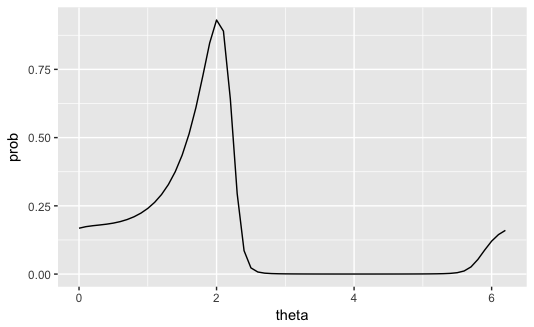
\includegraphics[clip,height= 35mm]{data/PN_sample1.png}
\end{center}
\caption{Projected Normal 分布の例}
\label{pnsample1}
\end{figure}

\end{frame}

\begin{frame}{背景}

\begin{itemize}

\item 方向データの確率分布として, よく用いられている von Mises Fisher 分布は二峰性のような分布の構造を表すことが出来ない.

\item  Projected Normal 分布は二峰性のような分布の構造を表すことが出来るので, 複数の最頻値を持つような方向データに対しても, 確率分布として表すことができる.

\end{itemize}

\begin{figure}[h]
 \begin{tabular}{c}
 \begin{minipage}{0.5\hsize}
  \begin{center}
   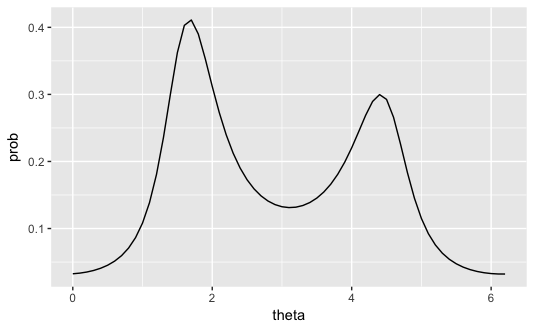
\includegraphics[clip,height= 35mm]{data/PN_sample2.png}
  \end{center}
  \caption{二峰性を持つ PN 分布の例}
  \label{pnsample2}
 \end{minipage}
 \begin{minipage}{0.5\hsize}
  \begin{center}
   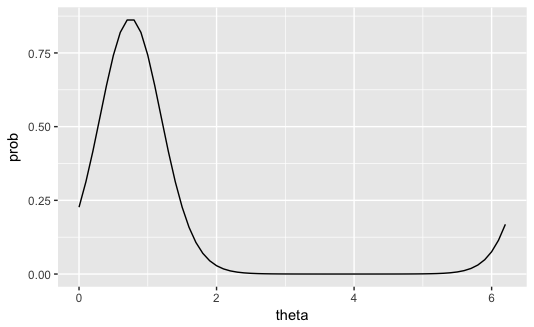
\includegraphics[clip,height= 35mm]{data/vonMises_sample.png}
  \end{center}
  \caption{Von Mises 分布の例}
  \label{vmsample1}
 \end{minipage}
\end{tabular}
\end{figure}

\end{frame}

\section{目的}
\begin{frame}{目的}
\begin{block}{目的}
\begin{itemize}
\item%%%%%%%%%%%%%%%%% ましなことを書きましょう笑 %%%%%%%%%%%%%%%%%%%%%%%%%%
複数の最頻値をもつ方向データを, 元データより少ないクラスターで説明することで、、、?
\end{itemize}
\end{block}
\end{frame}

\section{Projected Normal 分布}
\begin{frame}{Projected Normal 分布}

共分散行列が単位行列でない場合の, 円形の Projected Normal 分布の密度関数は以下の式で表せる. \cite{PN1}

\begin{eqnarray*}
\label{PNC}
p(\theta|\mu, \Sigma) = \frac{1}{2\pi A(\theta)}|\Sigma|^{-\frac{1}{2}}
\exp(C)\left\{1 + \frac{B(\theta)}{\sqrt{A(\theta)}} \frac{\Phi \left(\frac{B(\theta)}{\sqrt{A(\theta)}}\right)}{\phi \left(\frac{B(\theta)}{\sqrt{A(\theta)}}\right)}\right\} I_{[0,2\pi)}(\theta)
\end{eqnarray*}

$u^T = (\cos\theta,\sin\theta), A(\theta) = u^T\Sigma^{-1}u, B(\theta) = u^T \Sigma^{-1} \mu, C = -\frac{1}{2} \mu^T \Sigma^{-1} \mu$であり, $I_{[0,2\pi)} (\cdot)$は指示関数, $\Phi(\cdot),\phi(\cdot)$ は標準正規分布の確率密度関数と累積密度関数である.

\end{frame}

\section{混合 Projected Normal 分布}
\begin{frame}{混合 Projected Normal 分布}
%%% なんかさみしい。。

Projected Normal 分布の混合分布は以下のように定式化できる. 

\begin{eqnarray*}
\sum^J_{j=1} w_j \mathcal{PN}_2(\mu_j, \Sigma_j)
\end{eqnarray*}
\end{frame}

\section{シュミレーション}
\begin{frame}{シュミレーション(1/3)}

\begin{itemize}
\item
複数のvon Mises 分布に従う乱数を発生させて, 1つのデータにまとめることで混合データを作成する.

\item
Mixture von Mises 分布 および Mixture Projected Normal 分布による混合分布の推定を行う.
\end{itemize}

\vspace{-0.3cm}
\begin{figure}[H]
\begin{center}
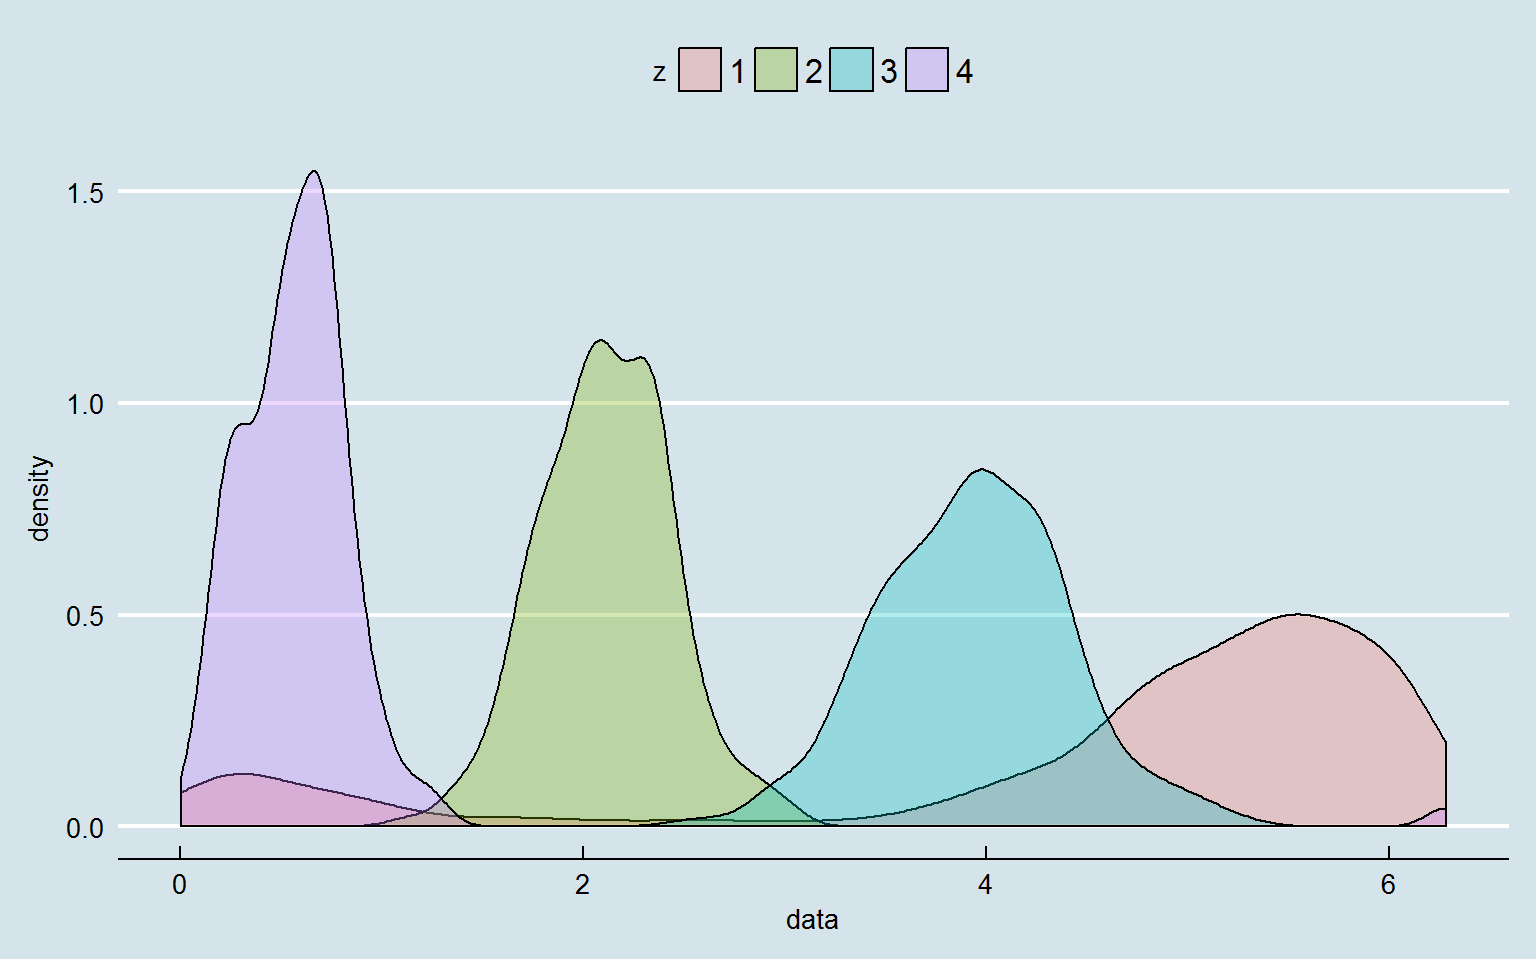
\includegraphics[clip,height= 35mm]{data/mix_test_data.png}
\end{center}
\caption{混合データ(クラスター数:4)}
\label{mixdata}
\end{figure}

\end{frame}

\begin{frame}{シュミレーション(2/3)}

\begin{itemize}
\item
得られた混合分布は, ともに元の分布の特徴をとらえている元になった.

\item
Mixture von Mises 分布では元のデータと同じく4つの元となる分布を推定したが, Mixture Projected Normal 分布においては3つの元となる分布により以下の結果が得られた.

\end{itemize}

\vspace{-0.3cm}
\begin{figure}[h]
 \begin{tabular}{c}
 \begin{minipage}{0.5\hsize}
  \begin{center}
   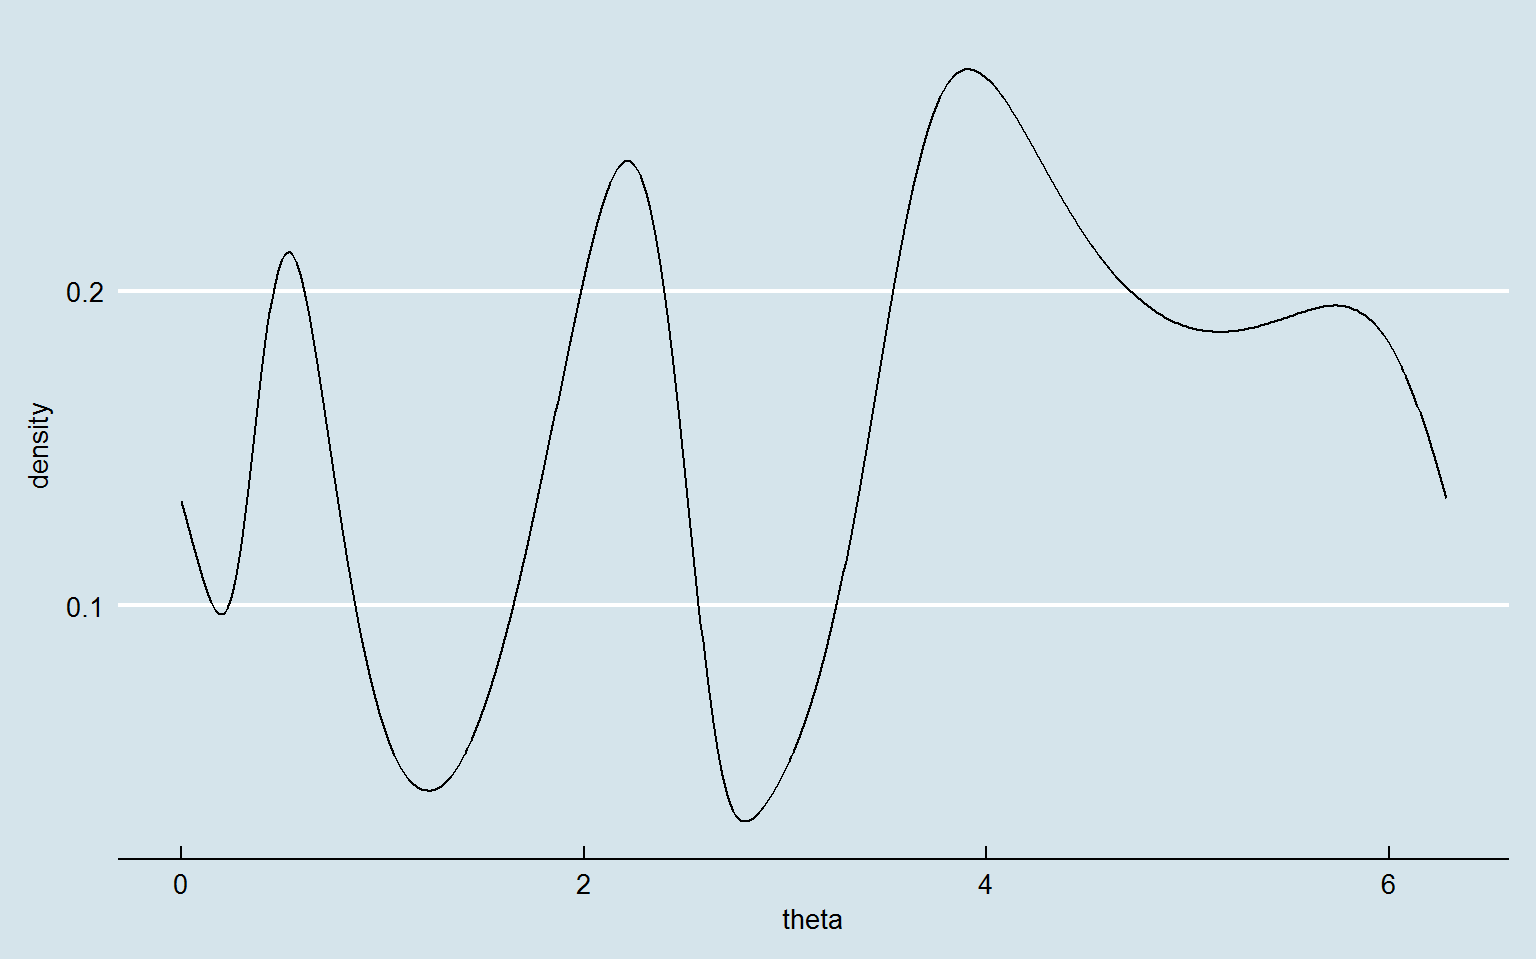
\includegraphics[clip,height= 35mm]{data/mix_pn.png}
  \end{center}
  \caption{Mixture Projected Normal 分布により推定した混合分布}
  \label{pnmix}
 \end{minipage}
 \begin{minipage}{0.5\hsize}
  \begin{center}
   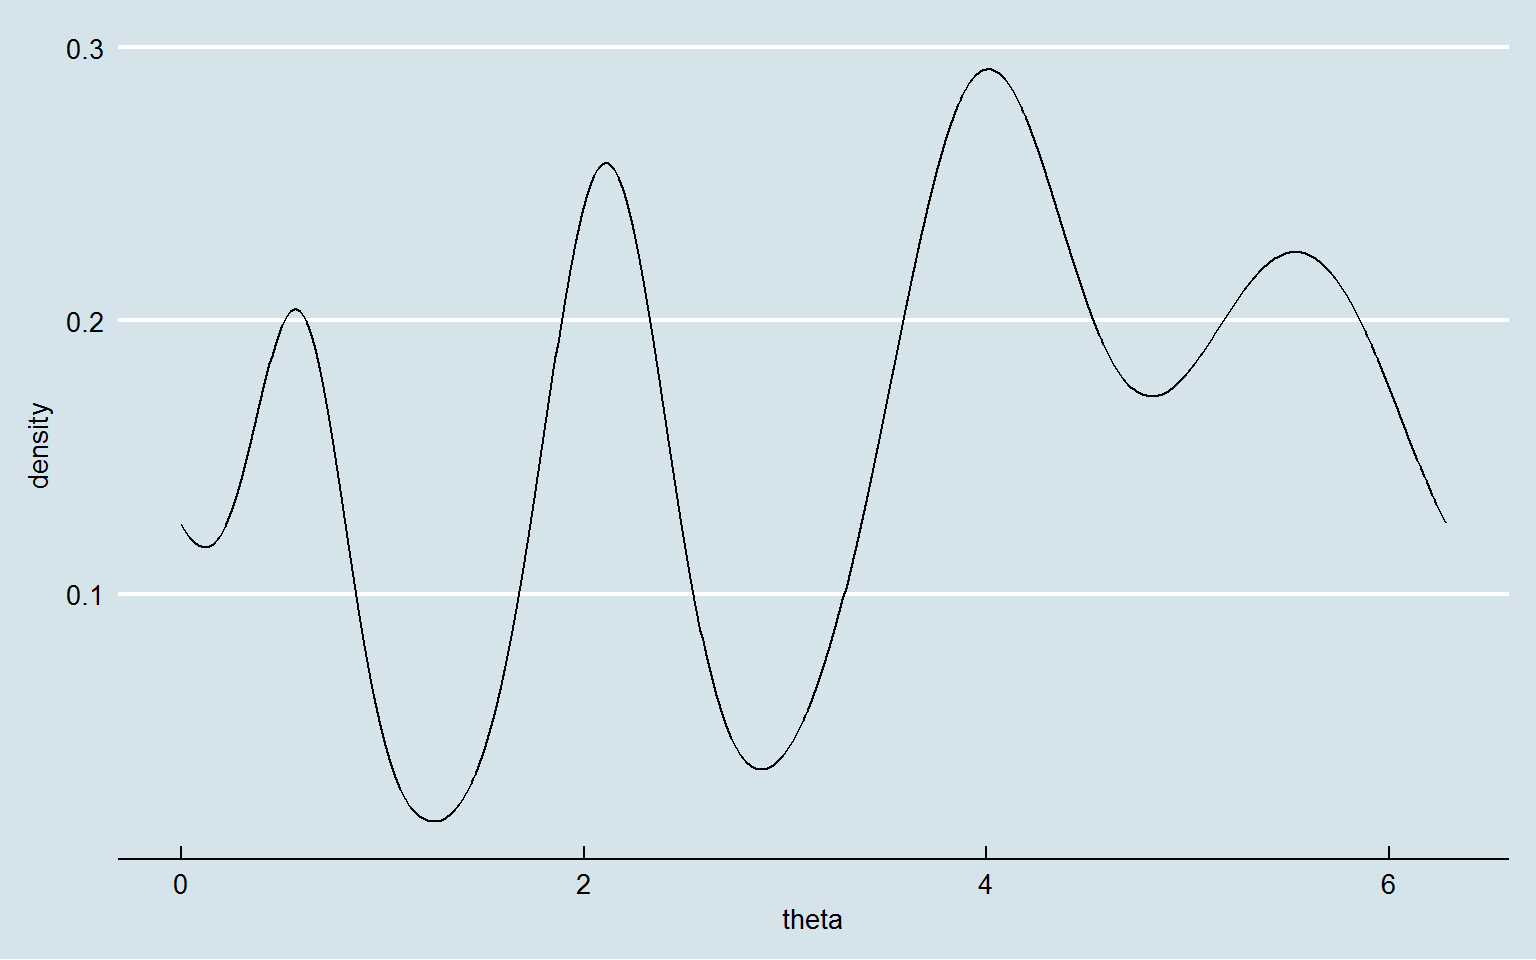
\includegraphics[clip,height= 35mm]{data/mix_von.png}
  \end{center}
  \caption{Mixture von Mises分布により推定した混合分布}
  \label{vonmix}
 \end{minipage}
  \end{tabular}
\end{figure}

\end{frame}

\begin{frame}{シュミレーション(3/3)}

\begin{itemize}

\item
混合分布を構成する, 各分布を推定する.

横軸が実際のクラスターで, 縦軸が予測のクラスターにおける分布である.

\end{itemize}

\begin{table}[H]
\begin{center}
\begin{tabular}{cc}

% 1
\begin{minipage}{0.5\hsize}
\begin{center}
\caption{PN 分布によるクラスター推定}
\begin{tabular}{c|c|c|c}
\hline
  & 1 & 2 & 3 \\ \hline \hline
1 & 38 & 10 & 352 \\
 2 & 1 & 192 & 7 \\
 3 & 0 & 2  & 298 \\
 4 & 93 & 0 & 7 \\
\hline
 \end{tabular}
 \end{center}
\end{minipage}

% 2
\begin{minipage}{0.5\hsize}
\begin{center}
\caption{VM 分布によるクラスター推定}
\begin{tabular}{c|c|c|c|c}
\hline
 & 1 & 2 & 3 & 4 \\ \hline \hline
1 & 333 & 10 & 39 & 18 \\
2 & 7 & 192 & 1 & 0 \\
3 & 298 & 2  & 0 & 0 \\
4 & 0 & 1 & 94 & 5 \\
\hline
\end{tabular}
\end{center}
\end{minipage}

\end{tabular}
\end{center}
\end{table}

\end{frame}

\section{データ解析}
\begin{frame}{データ解析}

\begin{itemize}

\item
気象庁が発表している風向データを用いて, データ解析を行う.\cite{amedas}

気象庁の風向データは36方位で記録されているので角度データ$(0 \leq \theta \leq 2 \pi)$ に変更して, 各分布の推定を行う.
\end{itemize}

\vspace{-0.3cm}
\begin{figure}[h]
 \begin{tabular}{c}
 \begin{minipage}{0.33\hsize}
  \begin{center}
   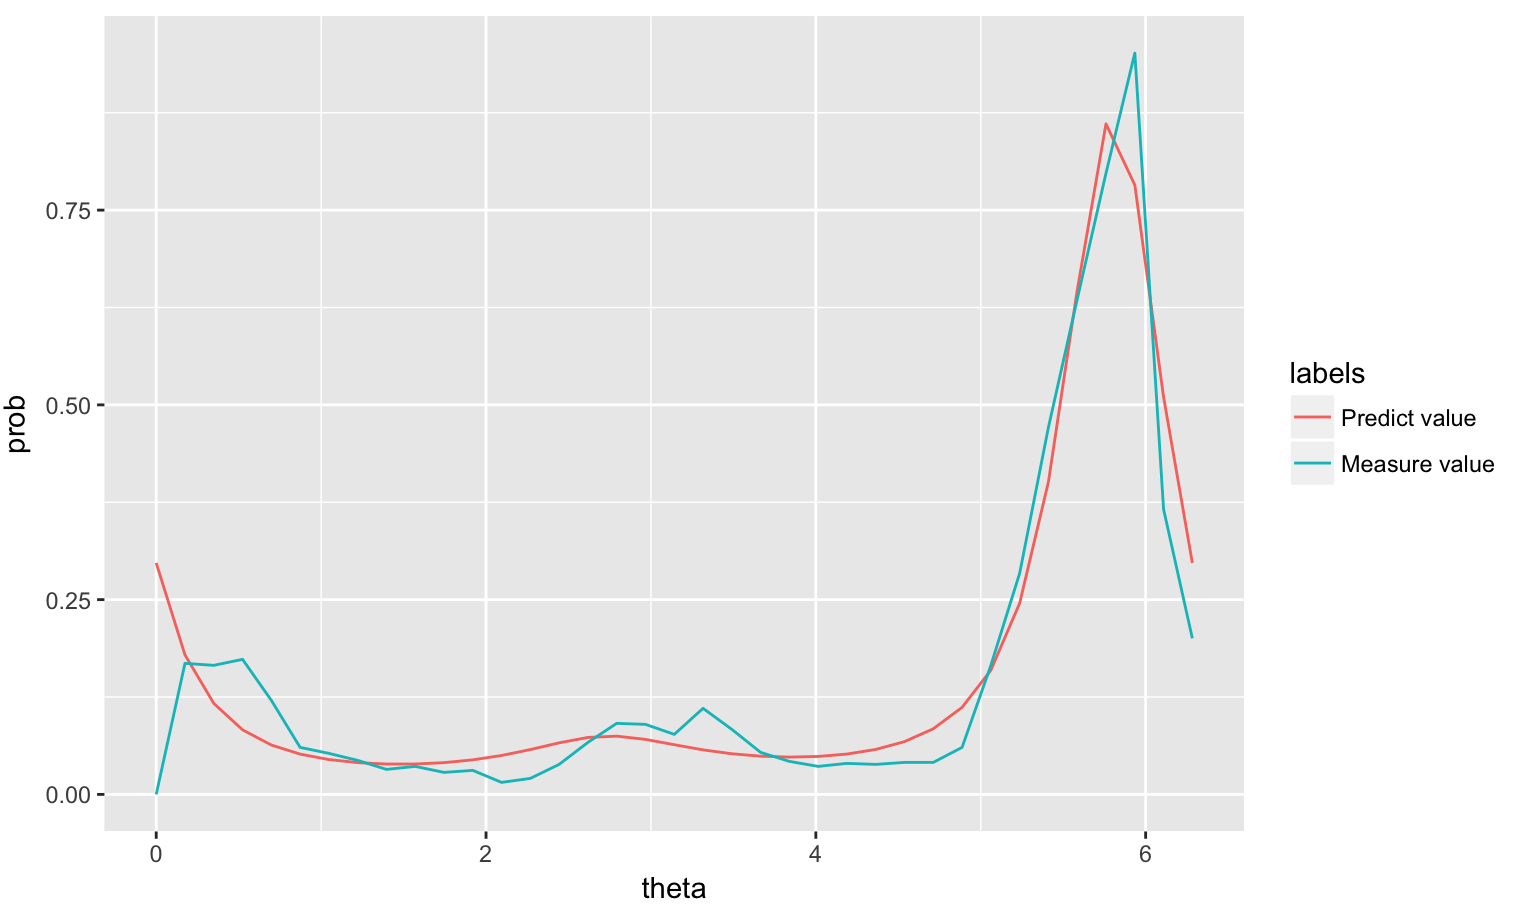
\includegraphics[clip,height= 25mm]{data/Tokyo_january.png}
  \end{center}
  \caption{東京(44132)の1月の風向データ}
  \label{pntokyo1}
 \end{minipage}
 \begin{minipage}{0.33\hsize}
  \begin{center}
   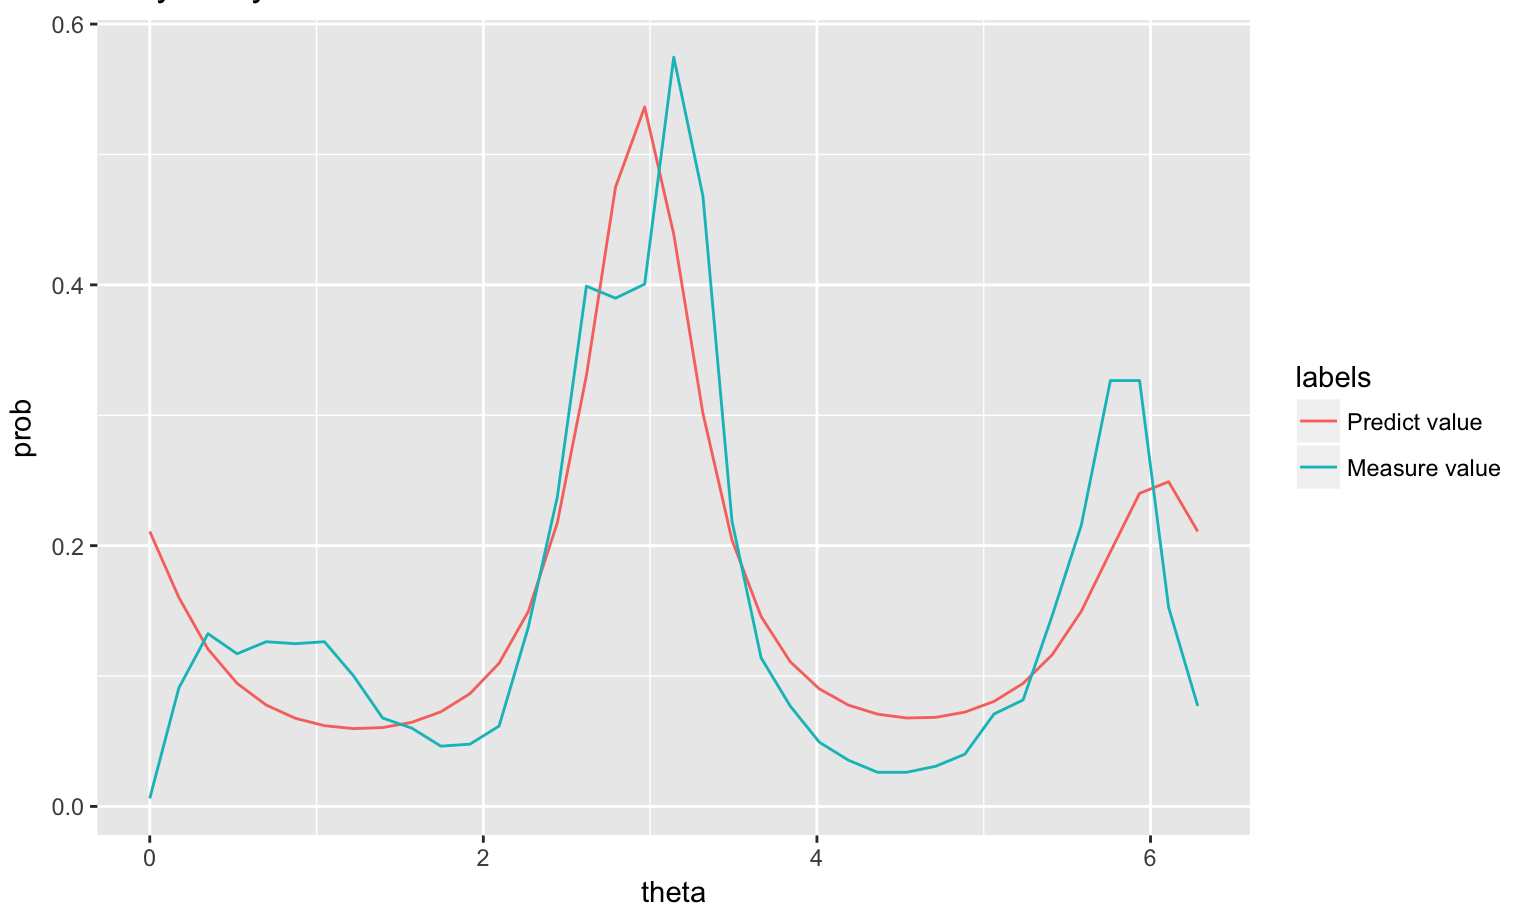
\includegraphics[clip,height= 25mm]{data/Tokyo_May.png}
  \end{center}
  \caption{東京(44132)の5月の風向データ}
  \label{pntokyo5}
 \end{minipage}
 \begin{minipage}{0.33\hsize}
  \begin{center}
   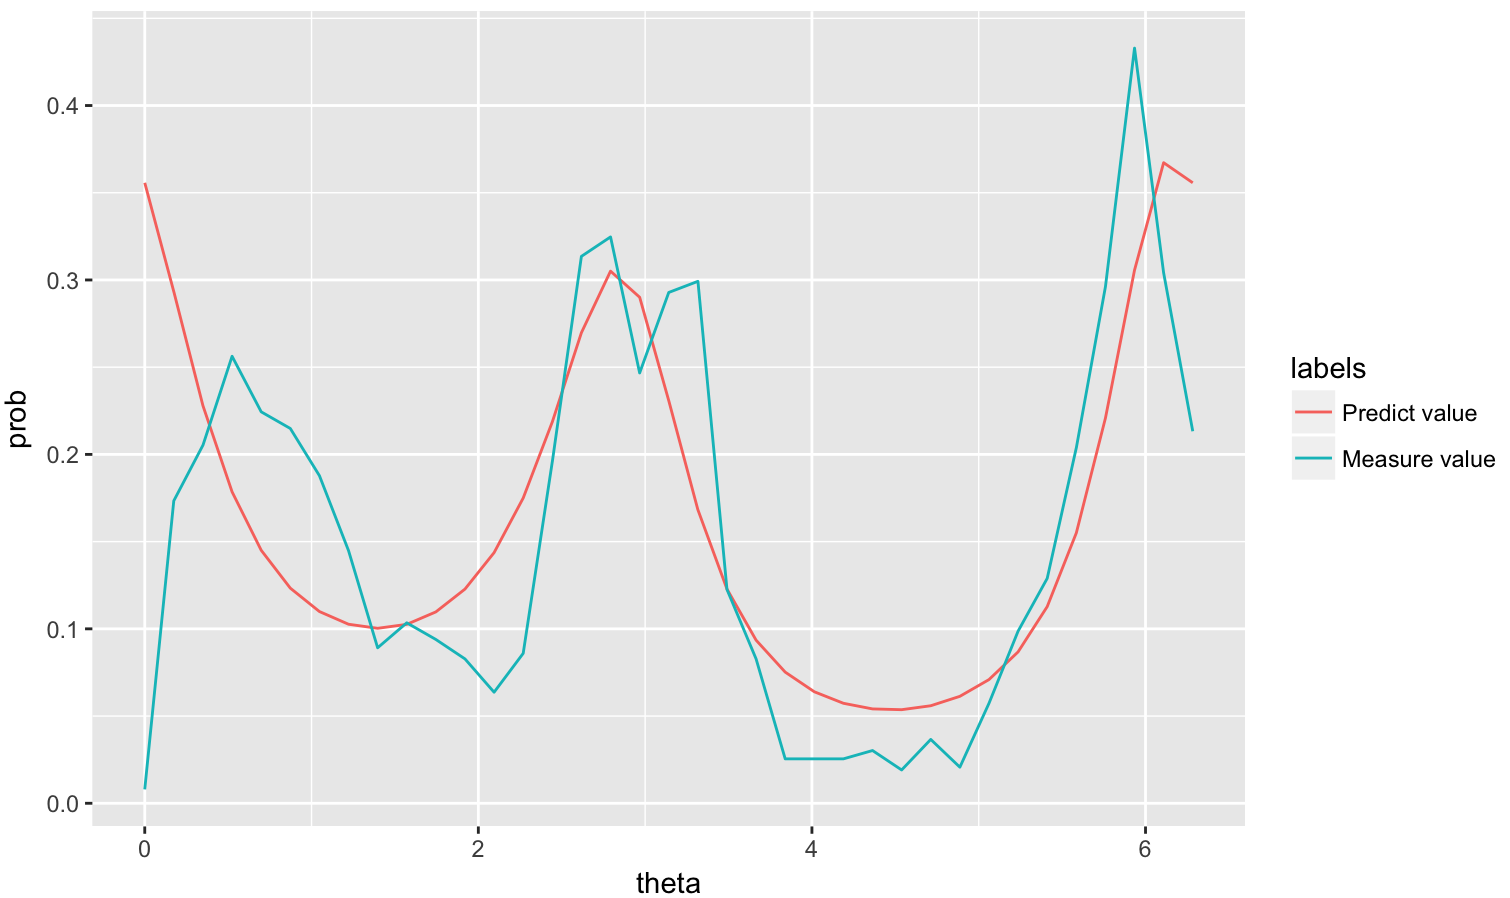
\includegraphics[clip,height= 25mm]{data/Tokyo_September.png}
  \end{center}
  \caption{東京(44132)の9月の風向データ}
  \label{pntokyo9}
 \end{minipage}
  \end{tabular}
\end{figure}

\end{frame}

\section{まとめと今後の課題}
\begin{frame}{まとめと今後の課題}

\begin{itemize}

\item
前日と前々日の混合分布で今日の風向の分布を予測.

\item
少数のデータで分布の予測.

\end{itemize}

\end{frame}

\section{参考文献}
\begin{frame}[allowframebreaks]{参考文献}

{\scriptsize
\begin{thebibliography}{99}
%\setlength{\itemsep}{-.5zw}
\beamertemplatetextbibitems %参考文献に番号を振る

\bibitem{GPN}
D.Hernandez-Stumpfhauser and F. Jay Breidt and Mark J. van der Woerd. (2017). The General Projected Normal Distribution of Arbitrary Dimension: Modeling and Bayesian Inference. {\it Journal of Bayesian Analysis}, Vol. 12, No. 1, pp. 113-133.

\bibitem{PN1}
Wang, F. and Gelfand, A. E. (2013). Directional data analysis under the general
projected normal distribution. {\it Statistical Methodology}, Vol.10, pp. 113-127.

\bibitem{PN2}
Gabriel Nunez-Antonio and Eduardo Gutierrez-Pena. (2005). A Bayesian Analysis of Directional Data using the Projected Normal Distribution. {\it Journal of Applied Statistics}, Vol. 32, No. 10, pp. 995-1001.

\bibitem{mvonMF}
Jalil Taghia and Zhanyu Ma and Arne Leijon. (2014). Bayesian Estimation of the von-Mises Fisher Mixture Model with Variational Inference. {\it IEEE}, Vol.36, No. 9, pp. 1701-1715.

\bibitem{amedas}
気象庁ホームページ(www.jma.go.jp/jma/kishou/info/coment.html) 

\end{thebibliography}
}

\end{frame}
\end{document}

%\vspace{-0.5cm}
%\begin{figure}[H]
% \begin{center}
 % 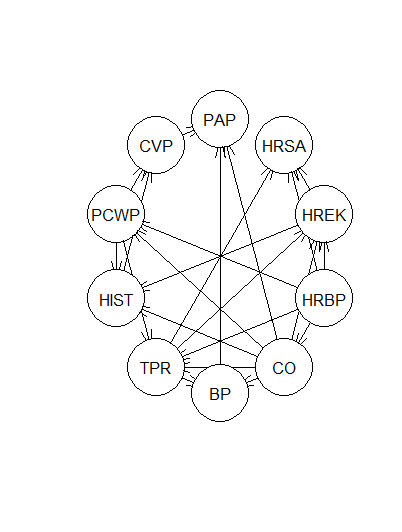
\includegraphics[width=40mm]{data/BN4.png}
 %\end{center}
 %\caption{ベイジアンネットワークの例}
 %\label{naive}
%\end{figure}